\documentclass[border=4pt,tikz]{standalone}
\usepackage{tikz}
\usetikzlibrary{arrows.meta,positioning,shapes.geometric}
\begin{document}
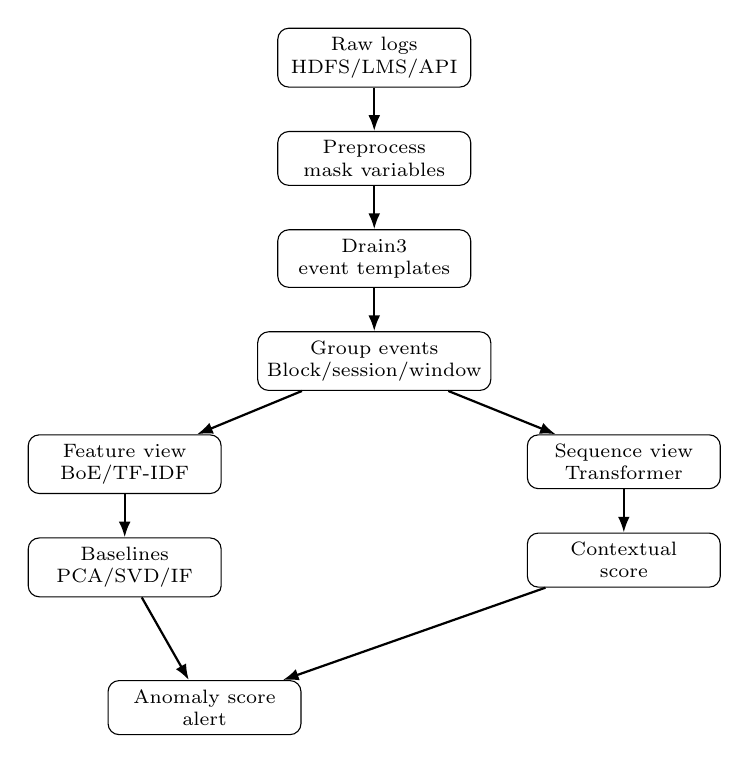
\begin{tikzpicture}[
    node distance=0.55cm and 0.45cm,
    box/.style={rectangle, draw, rounded corners, align=center, minimum width=2.45cm, minimum height=0.62cm, font=\scriptsize},
    arrow/.style={-{Latex[length=2mm]}, thick}
]
\node[box] (raw) {Raw logs\\HDFS/LMS/API};
\node[box, below=of raw] (pre) {Preprocess\\mask variables};
\node[box, below=of pre] (parse) {Drain3\\event templates};
\node[box, below=of parse] (seq) {Group events\\Block/session/window};
\node[box, below left=of seq] (vec) {Feature view\\BoE/TF-IDF};
\node[box, below=of vec] (base) {Baselines\\PCA/SVD/IF};
\node[box, below right=of seq] (bert) {Sequence view\\Transformer};
\node[box, below=of bert] (seqscore) {Contextual\\score};
\node[box, below right=1.05cm and -1.45cm of base] (score) {Anomaly score\\alert};
\draw[arrow] (raw) -- (pre);
\draw[arrow] (pre) -- (parse);
\draw[arrow] (parse) -- (seq);
\draw[arrow] (seq) -- (vec);
\draw[arrow] (vec) -- (base);
\draw[arrow] (seq) -- (bert);
\draw[arrow] (bert) -- (seqscore);
\draw[arrow] (base) -- (score);
\draw[arrow] (seqscore) -- (score);
\end{tikzpicture}
\end{document}
